% !TEX root = ../../mythesis.tex

\chapter{Background}
\label{chap:background}
    In this chapter, we introduce the reader to the background material necessary to understand the work conducted within this dissertation.
    We briefly highlight the technicalities of Ethereum blockchain and smart contracts, including common vulnerabilities in smart contracts.

\section{Ethereum}
    Ethereum is a blockchain technology that was introduced in 2014~\cite{wood2014ethereum}.
    A blockchain is basically a peer-to-peer network consisitng of computers as nodes that update and share a copy of one singular database without necessarily trusting one another.
    It can be said to be a specialized version of a cryptographically secure, transaction-based state machine.~\cite{wood2014ethereum}.
    The aforementioned database essentially acts as a ledger that keeps a record of every single transaction that the nodes perform within the blockchain network.
    The term “block” refers to the fact that transactions are grouped into batches;
    those batches are called “blocks”, data structures within the blockchain database where transaction data are permanently recorded.
    A transaction has to be included in such a block in order to be considered valid.
    The term “chain” refers to the fact that each block is cryptographically linked to its previous block via a cryptographic hash, whereby the first block (i.e., genesis block) counts as an exception as it has no previous block and therefore acts as a root of trust.
    In other words, blocks are chained together and form a chain of blocks, which is known as a “blockchain”.
    
    \begin{figure}
        \centering
        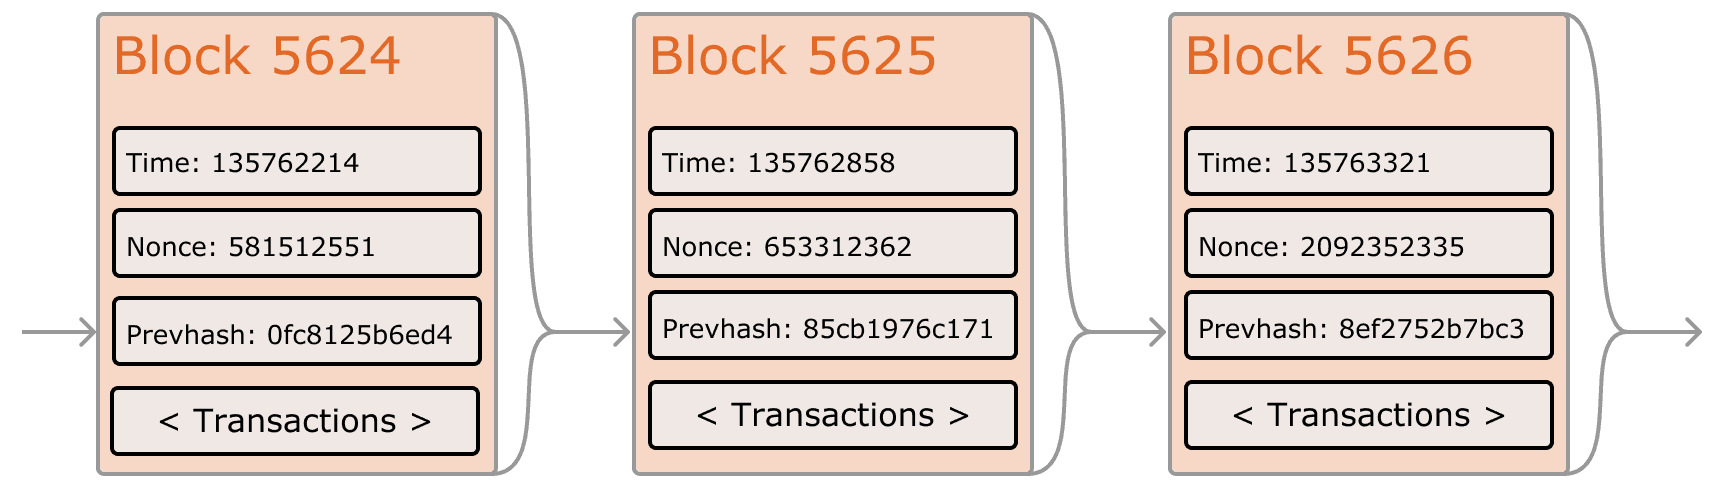
\includegraphics[width=\textwidth]{figures/ethereum-blocks.png}
        \caption{Ethereum blockchain structure.}
        \label{fig:ethereumBlockchainStructure}
    \end{figure}

    The Ethereum blockchain can be seen as a transaction-based, cryptographically secure state machine, that reads a series of inputs and, based on those inputs, transitions to a new state.
    Ethereum starts with a blank state called the “genesis state”.
    This genesis state transitions into a new state after executing a series of transactions.
    This new state represents the current state of the Ethereum blockchain, at any point in time.
    In other words, based on our analogy, blocks represent states and transactions represent state transitions.
    The data inside a block cannot be altered without changing all of its subsequent blocks.
    Changing all the subsequent blocks would require the consensus of the majority of the network.

    Every computer in the network must agree upon each new block and the chain as a whole.
    These computers are known as "nodes".
    Nodes act as an entry point to the blockchain and ensure everyone interacting with the blockchain has the same view on the data being recorded in the ledger.
    To accomplish this distributed agreement, blockchains make use of a consensus protocol.
    It is used to determine who is allowed to append the next block to the chain, and a random peer in the network has to be picked through it.
    Ethereum currently uses Proof-of-Work (PoW) as its consensus protocol.
    Proof-of-Stake (PoS) is another concensus protocol, for example.
    In order to append a new block to the blockchain, users have to generate a hash of the new block, which starts with a given number of zeros.
    Finding such a hash requires a lot of computing power.
    It acts as a “proof” that a node has done “work” by spending its computational resources.
    This process is known as mining and nodes which decide to participate in this process and try to create new blocks are known as miners.
    New blocks are then broadcast to the nodes in the network, checked and verified, thus updating the state of the blockchain for everyone.

    As participating nodes are allowed to propose new blocks simaltaneously and at nearly the same time, it can be the case that two or more blocks are proposed at once with a valid hash while referencing the same parent block.
    These competing branches that are created by these nodes are called “forks”.
    Blockchain forks pose a serious issue to Ethereum.
    They result in multiple concurrent states and make it difficult for the nodes to come to an agreement concerning which state should be the correct state.
    For example, if the states were to diverge, a user might own 100 coins on one chain, 200 on another, and 300 on another.
    Forks can happen intentionally or be deliberately orchestrated.
    To prevent multiple states and help determine which fork is the most valid one, Ethereum blockchain uses a technique known as the Greedy Heaviest Observed Subtree (GHOST) protocol.
    The GHOST protocol declares that of all the states, one must select the state that contains the most computation.
    One way to determine the heaviest state (computation-wise), is to look at the block number of the most recent block (i.e., leaf block) of a state, which amounts to the total number of blocks in the current state (not including the genesis block).
    The higher the block number, the longer the chain of that state and the greater the mining computation that must have gone into arriving at that current leaf block.
    This allows the blockchain nodes to agree on an accpeted version of the current state of the blockchain.
    Those blocks that are not included in the canonical chain are often referred to as orphans or uncle blocks.
    Unlike other blockchains, such as Bitcoin, Ethereum also adds uncle blocks to the aforementioned calculation to figure out the longest and computationally heaviest chain of blocks.
    This allows for the inclusion of more transactions and attributes a reward to the creators of uncle blocks as well as miners for declaring concurrent blocks as uncles and thereby keeping forked chains as short as possible.

    \begin{figure}
        \centering
        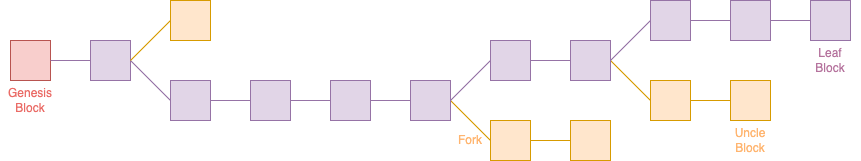
\includegraphics[width=\textwidth]{figures/uncle.png}
        \caption{An illustration of Ethereum's GHOST protocol.}
        \label{fig:uncle}
    \end{figure}

    \subsection{Ether}
        Ether is the native cryptocurrency of Ethereum.
        A cryptocurrency is a digital currency that is secured by means of cryptographic primitives.
        The purpose of ether is not only to allow users to exchange value between one another, but also to provide an economic incentive for users of its underlying platform to provide computational resources to the Ethereum network.
        Any network participant who sends a transactions must offer some amount of ether to the Ethereum network as a fee.
        This remuneration will be awarded to whoever gets to mine the block that includes the transaction, as a result of doing the work of verifying, executing, and broadcasting the transaction to the rest of the blockchain network.
        The amount of ether offered in such transaction as the corresponding fee, must correspond to the time and effort spent in executing the transaction.
        These costs prevent malicious participants from intentionally blocking up the network by requesting the execution of infinite computation or other resource-intensive actions, as these ill-intentioned participants must pay for the computation.

        Ethereum provides a metric system of denominations to describe different units of ether.
        Each denomination has its own unique name.
        Wei and Gwei are the most popular denominations.
        Wei is the smallest possible denomination of ether also known as the base unit, and as a result, many technical implementations base all their calculations in wei.
        Gwei (short for gigawei) is often used to describe costs related to “gas”.

    \subsection{Accounts}
        The global state of Ethereum is composed of many objects called “accounts”.
        They are able to interact with one another through so-called “messages”.
        Each account has a 20-byte address and a state associated with it.
        An address in Ethereum is a 160-bit identifier (a string of 42 hexadecimal characters) that is used to uniquely identify any account on the blockchain.
        There exist two different types of accounts (see Figure 2.4):
        
        \begin{itemize}
            \item \textbf{Externally Owned Accountss} (EOAs), which are controlled by private keys and have no code associated with them.
            \item \textbf{Contract Accounts} (CAs), which are controlled by their contract code and have code associated with them (i.e., smart contracts).
        \end{itemize}

        Both account types have the ability to receive, hold and send ether.
        EOAs can send messages to other EOAs and CAs by creating a transaction and signing it using their private key.
        The code that is associated with a CA, is executed whenever it receives a message from an EOA or a CA.
        The code allows a CA to perform various actions (e.g., write to storage, perform computations, etc.), which a EOA is not capable of.
        However, unlike EOAs, CAs cannot initiate new transactions on their own.
        Instead, CAs can only trigger messages in response to other messages that they have received from either an EOA or another CA.
        Thus, any actions that occurs on the Ethereum blockchain, are always set in motion by transactions that are triggered by EOAs.
        The account state consists of four fields, which are always present regardless of the type of account:

        \begin{itemize}
            \item \textbf{Nonce:} A number that acts as a simple counter which indicates the number of transactions sent from the account.
                This prevents the replaying of transactions and ensures that transactions are only processed once. If the account is an EOA, this number represents the number of transactions sent from the EOA's address. If the account is a CA, the nonce represents the number of contracts created by the CA.
            \item \textbf{Balance} The amount of cryptocurrency owned by this address in units of wei.
                Wei is the smallest subunit of ether (1 wei is equivalent to 10-18 ether).
            \item \textbf{Storage Root} A hash of the root node of the Merkle Patricia tree that encodes the storage contents of the account.
            This value is by default empty for both types of accounts and is solely updated for CAs whenever data is written to storage.
            \item \textbf{CodeHash} A hash of the bytecode associated with this account.
                For CAs, this represents a hash of the code that is stored on the blockchain. For EOAs, the this value is the hash of the empty string.
        \end{itemize}

        Creating an EOA has no cost as no data such as code, storage or balance is associated with the account at creation time.
        A CA on the other hand, has a cost because it uses the blockchain's storage to persist the contract code and data directly at creation time.

    \subsection{Transactions}
        Transactions are essentially cryptographically signed instructions from EOAs to update the state of the Ethereum blockchain.
        EOAs sign their transactions using their private key in order to cryptographically prove that the transaction could only have come from them and not from someone else.
        Two types of transactions exist: message calls and contract creations.
        The latter are transactions with an empty recipient field that result in creating new CAs (i.e., smart contracts). 
        The code, to be associated with the CA, is placed inside the data field of the transaction.
        Regardless of their type, all transactions contain the following fields:
            \begin{itemize}
                \item A count on the number of transactions sent by the sender. This number is incremented by one every time a transaction is sent by the sender.
                \item The amount of wei that the sender is willing to pay for each unit of gas that is used during the execution of the transaction.
                \item The maximum amount of gas units that the sender is willing to spent for the execution of this transaction.
                    This amount is set and paid upfront, before any computation is performed.
                \item The address of the recipient. If the recipient is an EOA, the transaction will transfer value, if the recipient is a CA, the transaction will transfer value as well as execute the contract's code.
                    A transaction with an empty recipient address is used to trigger the creation of a new CA.
                \item The amount of wei to be sent from the sender account to the recipient account.
                    Interestingly, this value may be used to set the starting balance of the newly created CA in a contract-creating transaction.
                \item These values represent the digital signature (R, S) which can be used to recover the public key (V).
                    These values identify the sender of the transaction and confirms that the sender has authorized the transaction.
                \item This field is only part of contract-creating transactions and consists of an unlimited length byte array that includes the code to be used during the initialization process and the code to be permanently associated with the newly created CA.
                \item This is an optional field that is only part of message calls and consists of a byte array of unlimited size that specifies the input data (e.g., , function name, function parameters) of the message call.
            \end{itemize}
            As previously mentioned, contract-creating transactions and message calls are always initiated by EOAs.
            However, this does not mean that CAs cannot communicate with other CAs.
            CAs can send messages or so-called “internal transactions” to other CAs.
            Internal transactions are similar to normal transactions, with the major difference being that they are not initiated by EOAs, but instead they are initiated by CAs.
            Moreover, internal transactions merely exist as virtual objects that, unlike transactions, are not persisted in the Ethereum blockchain and only exist at execution time.
            When a CA sends an internal transaction to another CA, the code that is associated with the recipient CA is executed.
            In contrast to normal transaction, internal transactions do not contain a gas limit by default.
            They are only limited by the gas limit that was determined by the normal transaction that triggered them.
            Thus, the gas limit that the EOA provides within its normal transaction, must be large enough to perform the execution of the normal transaction, including any sub-executions that occur as a result of that transaction, such as any internal transactions.
            If the execution of an internal transaction runs out of gas, then its execution will be will be reverted, along with any subsequent internal transactions triggered by the execution.
            However, the parent execution is not reverted.


    \subsection{Blocks}

        Blocks are batches of transactions with a reference to the hash of the previous block.
        This adds immutability and makes fraud noticeable, since a change in a transaction would invalidate all the previous blocks as all previous block hashes would change as well.
        Moreover, by grouping transactions into blocks, all network participants are given enough time to come to consensus, even in the case where hundreds of transactions are broadcast per second.
        The size of a block is usually bounded to a target size of 15 million gas units.
        However, the size of blocks will be increased or decreased depending on the demands of the network, up to a block limit of 30 million gas units (2x target block size).
        The total amount of gas spent by all transactions contained within the block must be less than the block gas limit.
        This is crucial as otherwise blocks could grow arbitrarily large and congest the blockchain.
        A block consists of a block header, a list of transactions, and a list of the block headers of the block's ommers.
        A block header consists of the following fields:

        \begin{itemize}
            \item \textbf{ParentHash}: A hash of the parent (previous) block's header (i.e., the pointer that links blocks together in a chain).
            \item \textbf{OmmersHash}: A hash of the current block's list of ommers. An ommer is a block whose parent is equal to one of the current block's parent's parent.
            \item \textbf{Beneficiary}: The account address that receives the fees for mining this block.
            \item \textbf{LogsBloom}: A Bloom filter (i.e., a data structure) that allows efficient querying of information contained in the logs.
            \item \textbf{Difficulty}: The effort required to mine this block.
            \item \textbf{Number}: The count of the current block. The block number of the genesis block starts at number zero and each subsequent block number is increased by one.
                The block number is often referred as the length of the blockchain in blocks.
            \item \textbf{GasLimit}: The current gas limit per block. This value represents the limit set on the overall gas consumption for this block.
            \item \textbf{GasUsed}: The sum of the total gas used by all transactions contained in this block. This value cannot surpass the GasLimit.
            \item \textbf{Timestamp}: The UNIX timestamp when the block was mined.
            \item \textbf{ExtraData}: Arbitrary data that can set by the miner. This data is limited to 32-byte and usually refers to the name of the miner or the client version that was used to mine the block.
            \item \textbf{MixHash}: A hash that, when combined with the nonce, proves that this block meets the difficulty of this block.
            \item \textbf{Nonce}: A value that, when combined with the MixHash, proves that this block has performed the required work.
            \item \textbf{StateRoot}: The hash of the root node of the Merkle Patricia trie that stores the state of all accounts (i.e., account balances, storage, code, and nonces).  The hash is calculated only after all transactions have been executed.
            \item \textbf{TransactionsRoot}: The hash of the root node of the Merkle Patricia trie that stores all transactions listed in this block.
            \item \textbf{ReceiptsRoot}: The hash of the root node of the Merkle Patricia trie that stores the receipts of all transactions listed in this block.
                Transaction receipts are generated after the execution of a transaction contain information such as logs or the actual gas that has been used during execution.

        \end{itemize}

        Block times are much lower in Ethereum (~15 seconds) than compared to those of other blockchains, such as Bitcoin (~10 minutes).
        The block time refers to the time that it takes to mine a new block.
        In Ethereum, the average block time is evaluated after each block.
        The expected block time is set as a constant at the protocol level and is used to protect the network's security when miners gain more computational power.
        The average block time is compared with the expected block time, and if the average block time is higher, then the difficulty contained in the block header is decreased.
        If the average block time is smaller, then the difficulty in the block header is increased.
        A smaller average block time enables faster transaction processing.
        However, shorter block times also means that miners will be more likely to find more competing block solutions.
        These competing blocks are often referred as ommers or uncles and are seen as “orphaned blocks”, hence, blocks that were mined but are not part of the canonical chain.
        The purpose of ommers is to incentivise miners to include orphaned blocks as a part of the canonical chain and thereby avoid forks.
        Miners are only allowed to include orphaned blocks that are not more than six block numbers away from the current block number.

    \subsection{Ethereum Virtual Machine}
        The Ethereum Virtual Machine (EVM) is a purely stack-based, register-less virtual machine that runs low-level bytecode and supports a Turing-complete set of instructions.
        For a simple analogy, you can think if it like the Java programming langauge that uses the Java Virtual Machine (JVM).
        It represents the execution model of a virtual state machine, defining how the states in the Ethereum blockchain are changed.
        Every instruction is represented by a one-byte opcode (e.g., 0x60 → PUSH1, e.g., 0x50 → POP, etc.).
        The instruction set consists of more than 140 different instructions ranging from basic operations such as arithmetic operations or control-flow operations to more specific ones, such as the modification of a contract's storage or the querying of properties related to the executing transaction (e.g., sender) or the current blockchain state (e.g., block number).
        The EVM uses a memory model that is specific to the execution of smart contracts and differs from the traditional von Neumann architecture (see Figure 2.7). Instead of organizing code and data in one large general-pu
        EVM is activated whenever a Smart contract on the Ethereum blockchain needs to be executed by receiving a message or transaction.
        Execution of a contract in EVM does not need any external resources from the network or file system, but there may exist some external calls to the functions of the other contracts in the blockchain.
        
        Instead of organizing code and data in one large general-purpose memory, the EVM follows the Harvard architecture by separating code and data into four different address spaces: (1) an immutable code address space, which contains the smart contract's bytecode, (2) a mutable but persistent storage address space that allows smart contracts to persist their data across executions, (3) a mutable but volatile memory address space that acts as a temporary data storage for smart contracts during execution, and finally (4) a stack address space that allows smart contracts to pass arguments to instructions at runtime.

        The EVM employs a gas mechanism that assigns a cost to the execution of an instruction.
        This mechanism prevents DoS attacks and ensures termination by solving the halting problem.
        When issuing a transaction, the sender has to specify a gas limit and a gas price.
        The gas price defines the amount of ether that the sender is willing to pay per unit of gas used.
        As the gas price is coupled to ether, developers are motivated to write efficient programs to keep transaction costs low and to avoid “infinite” loops.
        The base fee for executing a transaction starts at 21,000 gas units.
        The final execution costs are determined by multiplying the gas price with the gas used.
        The gas limit is specified in gas units and must be large enough to cover the amount of gas consumed by the instructions during a contract's execution, otherwise execution will terminate abnormally with an out-of-gas exception and its effects will be rolled back.
        The EVM also throws an exception when a jump destination is invalid, an instruction does not exist, or when there are not enough elements on the stack to perform an given operation.

        Instructions operate on a stack of 256-bit big-endian words.
        The stack is private to a single contract (but not to methods within the contract) and is almost free to use in terms of gas.
        The size of the stack is limited to 1,024 items.
        In addition to the stack, smart contracts can also store variables in memory.
        Memory is a random-access array of 256-bit words that is accessible only by the currently executing smart contract.
        Memory is always initialized with zeros and thus isolated from previous executions.
        Memory is also used to pass arguments across message calls.
        Figure 2.8 shows an example of an EVM message call.
        The CALL instruction first copies the arguments of the message call from memory into the input data of a new instance of the EVM.
        The control is then returned back to the message caller via the RETURN instruction and the return value that includes the result of the message call is placed into the memory of the caller.
        Besides stack and memory, the EVM also features storage.

        While stack and memory are volatile and may only hold values during execution, storage is persistent and part of the world state $\delta$.
        It is organized as a Patricia Merkle trie holding sets of key-value stores for each account.
        Storage is isolated from other smart contracts and is the only way for a smart contract to retain state across executions.
        While storage is theoretically unlimited, its use is expensive (compared to stack and memory) and should only be used to store small amounts of data.

\section{Smart Contracts}
    The concept of smart contracts has been first introduced by Nick Szabo in one of his works in 1997.~\cite{szabo1997formalizing}
    According to Szabo, smart contracts combine protocols, users' interfaces, and promises expressed via interfaces over public networks.
    Szabo described the notion of a system consisting of automatic, self-executing computer programs that would facilitate the enforcement of clauses contained in legal contracts and reduce mental and computational transaction costs, imposed by either
    principals, third parties or their tools.
    It took years for efficient trustless systems like blockchains such as Ethereum to develop and grow in order for them to utilize the concept of smart contracts in full, hence the 20-year delay between the ideation and real-world implementation of them.

    \subsection{Solidity}
        Solidity is an object-oriented programming language and it is currently the most prominent programming language for developing smart contracts in Ethereum.
        Its syntax resembles a mixture of C and JavaScript, but it comes with a variety of unique concepts that are specific to smart contracts and might be unfamiliar or confusing for new developers, such as the visibility of function modifiers: internal, external, pure, view, the function-wide scoping of variables, the emitting of events, or smart contract specific operations such as selfdestruct or revert.
        Similar to C, Solidity uses a function dispatch table to select what function to execute during runtime.
        The compiler does so by adding to the bytecode a function dispatcher that first loads the hash of the name of the function to be executed (the initial 4 bytes of the transaction input data Id) into the stack and then jumps to the function implementation that is associated with the hash (see Figure 2.9).
        Now, unlike C and JavaScript, the concept of “undefined” or “null” values does not exist in Solidity.
        Newly declared variables always have a default value depending on their type.
        For example, integers are always initialized with zero, whereas Boolean's are always initialized with False.
        Besides common variable types, such as int, bool, or string, Solidity also provides unique types such as mapping or address.
        The variable type mapping behaves similar to a dictionary in Python by mapping keys to values and therefore allowing an easy access to storage.
        The variable type address is meant to hold addresses of Ethereum accounts and has member function such as balance, send, transfer, call, etc.
        The member functions send, transfer, and call can be used to move ether from one address to another.
        All these functions make use of the EVM CALL instruction, with difference being the gas limit that can be used and the behavior on an error.
        
        Almost all variable types in Solidity are of type value, meaning that their value is copied when passed as an argument to a function.
        In contrast, the value of variable types of type reference, are not copied and therefore modified across function calls.
        Currently, variable types of type reference comprise mappings, arrays, and structs.
        Developers always have to explicitly state the data area where the type is stored when using a variable of type reference: memory (where its lifetime is limited to an external function call), or storage (where its lifetime is limited to the lifetime of the contract).
        In general, state variables are always stored in storage, function arguments are always stored in memory, and local variables of type value are stored in the stack.
        Moreover, Solidity suggests to be a statically typed language, i.e., the compiler expects type information for each variable to be made explicit.
        For instance, integers can be signed and unsigned, and of lengths between 8 and 256 bits in 8-bit steps denoted as uint8 or int128.
        This resembles integer types in C and may lead novice developers to assume that a uint8 will occupy 8 bits in memory, while an int128 occupies 128 bits.
        However, this assumption is wrong. Any integer type will be represented inside the EVM as 256-bit values in big endian order using two’s-complement.
        That is, the integer type system of Solidity is not entirely consistent with that of the EVM, which can lead to programming errors.
        Explicit conversion between primitive types is possible, but the effects are not well documented.
        In fact, the documentation reads: Note that this may give you some unexpected behavior so be sure to test to ensure that the result is what you want.

        For example, explicitly casting a signed negative integer into an unsigned one will not result in the absolute value, but rather simply leave its bit-level representation intact.
        Interestingly, Solidity does not support floating points.
        However, similar to JavaScript, Solidity provides members such as length or push for arrays.

        Apart from variables, Solidity also provides units for ether and time (e.g., wei, days, etc.) as well as special keywords and functions which always exist in the global namespace and are mainly used as general-use utility functions or to provide information about the blockchain.
        Also mathematical and cryptographic functions are provided (e.g., addmod, ecrecover, etc.).
        For error handling, Solidity provides two convenience functions called assert and require, that can be used to check for a condition and to throw an exception if the condition is not met.
        Developers can interleave Solidity statements with inline assembly in a language called Yul, which is close to the one of the EVM.
        This gives more fine-grained control and bypasses optimizations imposed by the compiler.
        An inline assembly block is marked via the keyword assembly.
        The inline assembly code can access local Solidity variables, but different inline assembly blocks cannot call functions or access variables defined in a different inline assembly block.

    \subsection{Bytecode}
        Ethereum bytecode consists of a sequence of bytes that is interpreted by the EVM.
        Each byte either encodes an instruction or data.
        Figure 2.10 depicts the anatomy of Ethereum bytecode.
        Ethereum bytecode consists of two main parts: deployment bytecode and deployed bytecode.
        Deployment bytecode includes the deployment logic of the smart contract.
        This logic is responsible for initializing state variables and reading constructor arguments appended at the end of the Ethereum bytecode.
        It is also in charge of extracting the deployed bytecode from the Ethereum bytecode and copying it to persistent storage.
        This is achieved via the CODECOPY and RETURN instructions.
        Starting from a given offset and for a given size, the CODECOPY instruction first copies the code running in the current environment to memory.
        Afterwards, the RETURN instruction returns the code that has been copied into memory to the EVM.
        As a result, the EVM creates a new contract by generating a new 160-bit address and persisting the returned code with this new address.
        The deployed bytecode contains the runtime logic (i.e., runtime bytecode) and optional metadata.
        The runtime bytecode is the logic that is executed whenever a transaction is sent to a smart contract.
        Some compilers, such as the Solidity compiler, also append some metadata (e.g., compiler version) to the end of the runtime bytecode.

    \subsection{Vulnerabilities}
        Atzei et al.~\cite{atzei2017survey} were the first to publish a survey of smart contract vulnerabilities and their corresponding attacks.
        However, their survey goes back to 2016.
        Since then, several new vulnerabilities and attacks have emerged (e.g., Parity wallet hacks, integer overflows, etc.).
        In 2018, the NCC Group released their own inititative of ranking smart contract vulnerabilities, namely, the Decentralized Application Security Project (DASP).~\cite{dasp}
        It is an open and collaborative project to join efforts in discovering and documenting smart contract vulnerabilities within the security community.
        The idea is similar to the well known Open Web Application Security Project (OWASP).
        However, neither the ranking nor the list of vulnerabilities has been updated since its first release in 2018.
        Another initiative to document well-known attacks is the one presented by ConsenSys, called the Smart Contract Weakness Classification Registry (or simply SWC Registry).~\cite{swcregistry}
        It has been released with the goal to provide a common way to report and classify security issues in smart contracts.
        It loosely resembles the terminology and structure used in the Common Weakness Enumeration (CWE) project.
        Unfortunately, their list only contains a handful of vulnerabilities.
        At the time of writing, it includes 37 entries.
        Each entry consists of an identifier (SWC-ID), a weakness title, a CWE parent, and a list of related code samples.
        In 2019, Chen et al. ~\cite{chen2020survey} presented a survey of vulnerabilities, attacks, and defenses for the Ethereum blockchain.

        We provide in the following a detailed explanation of some of the more prominent smart contract vulnerabilities according to the above-mentioned DASP collection of vulnerabilities:

        \paragraph{Re-entrancy}
            A typical flaw in smart contracts are re-entrant calls.
            Re-entrancy may occur whenever a contract sends a value to or calls a function from another contract, and the called contract has enough gas to call back the original contract.
            As a result, the called contract re-enters the original contract.
            Therefore, the original contract must guarantee that its state is always correct, independent of re-entrant calls.
            Otherwise, a malicious contract can take advantage of an incorrect intermediate state to steal funds.
            The 2016 DAO hack remains the most famous example of a reentrancy attack not only because an unknown attacker managed to steal funds worth 50M USD [47], but also because it led to a hard fork of the Ethereum blockchain [164].
            A way to protect against reentrancy is to use the Solidity methods send or transfer rather than call.
            The aforementioned methods limit the amount of gas to 2,300 units, which makes it impossible for the called contract to modify the state or make any function calls.
            However, this only protects the sending of value.

        \paragraph{Access Control}
            A typical design pattern in smart contracts is to assign an address as the owner of the smart contract [107].
            This address has then privileged access to functions that can either update sensible variables, transfer funds, or destroy the entire contract.
            Unfortunately, this also means that faulty implementations of access control can lead to devastating consequences. One example of a flawed access control implementation is the use of Solidity's tx.origin to check whether the current address is authenticated to perform a sensible function call such as the withdrawal of funds.
            However, tx.origin does not represent the currently calling address, but the very first address that initiated the transaction.
            Remember that within a transaction, contracts can call other contracts, and therefore the calling address can be a different one at runtime.
            An attacker can perform a man-in-the-middle attack by first convincing a victim to send a transaction to the attacker's contract, which then performs within the same transaction a message call to the victim's wallet.
            If the wallet checks for the transaction origin to authenticate users, then the attacker will be authenticated as the victim and might be able to steal the funds.
            Developers should, therefore, rely on the msg.sender property to authenticate user accounts.

        \paragraph{Bad Randomness}
            Randomness is hard to achieve in general. In Ethereum it is even harder, since smart contracts are executed in a deterministic way.
            However, games and lotteries sometimes require non-deterministic values. Therefore, a variety of smart contracts rely on “unpredictable” information originating from yet unmined blocks, such as blockhash or number. They most often use this information as a seed to generate pseudo-random numbers. However, because the sources of randomness are predictable, malicious users can brute force the values of blocks before they have been mined.
            The Run [43] and SmartBillions [69] are famous examples of smart contract lotteries using block information for generating random numbers.
            In October 2017, an attacker was able to exploit the predictability of block information and steal 400 ether from the SmartBillions contract [84].

        \paragraph{Frontrunning}
            Users observing the network can see and react to transactions before they are mined. Miners typically order transactions based on their gas prices.
            This results in gas price wars between users in the network.
            Frontrunning is therefore also known as transaction order dependence (TOD).
            A decentralized exchange is a perfect example on how this can be exploited. An attacker observes a transaction containing a large buy order and quickly broadcasts its own transaction containing a buy order with a larger gas price in order to be executed before the observed buy order.
            A few other cases related to frontrunning have been studied by Eskandari et al.~\cite{eskandari2019sok}
            Common mitigations against frontrunning include the use of commit and reveal schemes or the specification of a minimum or maximum acceptable price range on a trade, thereby limiting price slippage.
        
        \paragraph{Time Manipulation}
            Sometimes smart contracts need to rely on the current time to either be able to accomplish their defined task, such as locking a token sale, or unlocking funds at a specific time in a game.
            In Solidity, the current timestamp is retrieved via \texttt{block.timestamp} or \texttt{now}.
            However, this value can be set by miners and can be manipulated.
            If a miner holds enough value inside a smart contract, then the miner could gain an advantage by choosing a suitable timestamp for a block that he or she mines.
            Smart contracts should, therefore, avoid relying on timestamps originating from blocks.
            Atzei et al. stated that the ponzi smart contract GovernMental is vulnerable to a timestamp manipulation attack~\cite{atzei2017survey}.
            However, there is no reported incident of such an attack in the wild.
        
        \paragraph{Short Address}
            Short address attacks are a side-effect of the EVM itself accepting incorrectly padded arguments. 
            Function arguments are typically encoded as 32-byte chunks of data within the input field of an Ethereum transaction.
            However, if the length of an encoded argument is shorter than 32 bytes, then EVM will auto-pad extra zeros to the end of the argument so that it always has a length of 32 bytes, no matter the size of the original encoding.
            Attackers can exploit this vulnerability by generating specially-crafted addresses that end with trailing zeros.
            The EVM does not check the validity of addresses, and the only way to prevent this attack is to check the length of a transaction's input at smart contract scope using \texttt{msg.data}.
